% !TEX root = main.tex
% --+ 11.31 SUMMARY +-----------------------------------------------------------
% The energy deposited by electrons in the active area of the calorimeters is a fraction of their total energy, $E_\text{tot}$.
% This value is proportional to their momentum, $P$, for energies above a few hundred MeV.
% Heavier particles, due to their reduced penetration capabilities, tend to lose an amount of energy independent of their momentum.
% The electron sampling fraction measures the amount of energy lost depending on the momentum of a particle.
% This allows for both the measurement of the electron's energy and the differentiation of electrons from other particles \cite{wigmans2000}.
%
% To obtain the sampling fraction, the hits of each calorimeter by itself (PCAL, ECIN, and ECOU) are separated into arrays, with an additional array containing the union of the other three.
% Then, these arrays of hits are separated into 20 momentum bins.
% Each bin has a size of 0.4 GeV, starting at 1.0 GeV and ending at 9.0 GeV.
%
% 1-dimensional histograms are then created from the data in these arrays, measuring the deposited energy divided by the vertex momentum ($E/p$).
% A Gaussian fit plus a quadratic background is then applied, following the function described as
%
% \begin{equation*}
%     f(x) = p_0 g(x, \mu, \sigma) + p_1 x^2 + p_2 x + p_3, \hspace{12pt}
%     \text{where} \hspace{4pt}
%     g(x, \mu, \sigma) = \frac{1}{\sigma \sqrt{2\pi}} \exp \left(-\frac{1}{2} \frac{(x - \mu)^2}{\sigma^2}\right),
% \end{equation*}
%
% where $\mu$ and $\sigma$ represent the mean and standard deviation of the distribution, respectively. The fit is limited to the range between $0.15$ and $0.30$ for the expected $E/p$ values for electrons based on theory.
%
% Examples of these plots are shown in Figure \ref{fig::13.30::sampling_fraction_fit_1d}.
% From the figure, it can be observed that there are not enough electrons in the extreme momentum ranges, such as from $1$ to $1.4$ GeV or from $8.6$ to $9$ GeV.
% Consequently, the sampling fraction fit, described in Equation \eqref{eq::13.30::sampling_fraction_fit_2d}, only considers data within the range of $1.4$ to $8.6$ GeV.

\begin{frame}{Sampling Fraction Estimation}
    \label{11.31::sampling_fraction_estimation}

    To estimate the \ef{sampling fraction} (\% of energy deposited by $e^-$ on calorimeters), we fit \ef{$E_{dep}/p$} distributions in 0.4 GeV \ef{$p$} bins to
    \begin{empheq}[box={\eqbox[5pt][5pt]}]{equation*}
        f(x) = p_0 \cdot g(x, \mu, \sigma) + p_1 x^2 + p_2 x + p_3,
    \end{empheq}
    where \ef{$g(x, \mu, \sigma)$} is a Gaussian distribution with mean \ef{$\mu$} and standard deviation \ef{$\sigma$}.

    \vspace{-12pt}

    \begin{columns}[onlytextwidth,T]

    \begin{column}{.49\linewidth}
        \begin{center}
            \begin{figure}[t]
                \centering{
                    \fbox{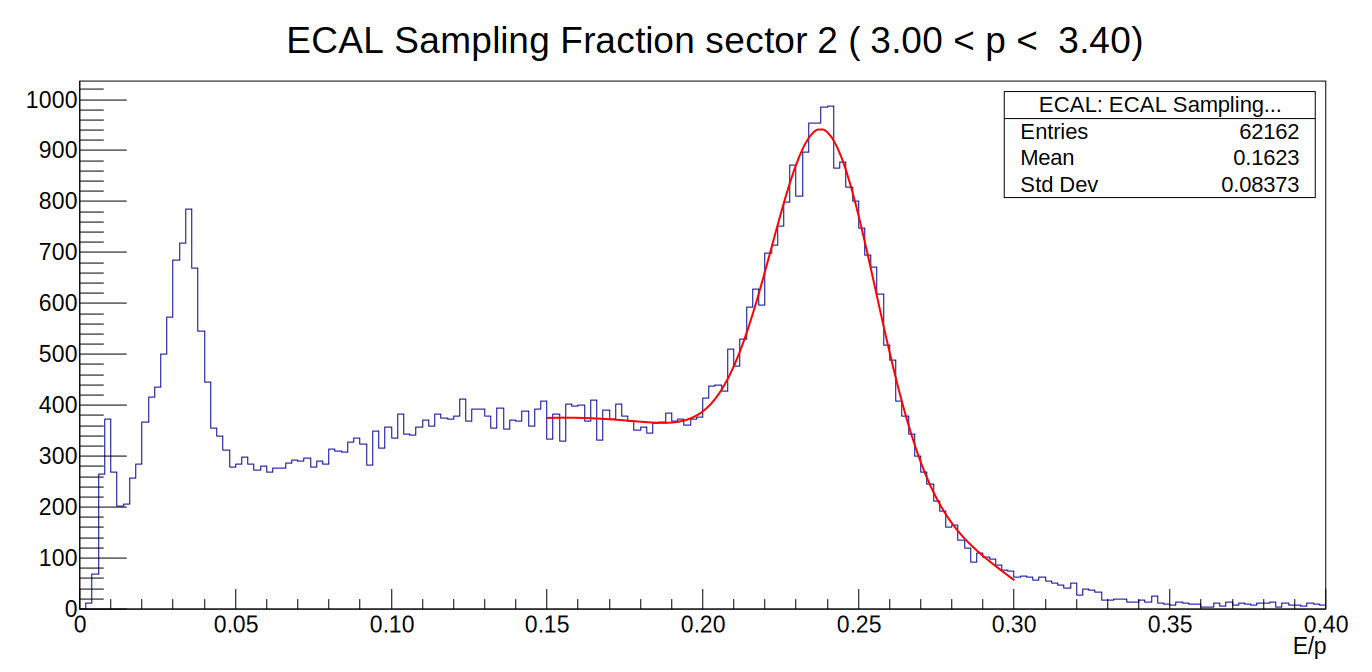
\includegraphics[width=\textwidth]{31sf_1d_plot1.pdf}}
                }
            \end{figure}
        \end{center}
    \end{column}

    \begin{column}{.49\linewidth}
        \begin{center}
            \begin{figure}[t]
                \centering{
                    \fbox{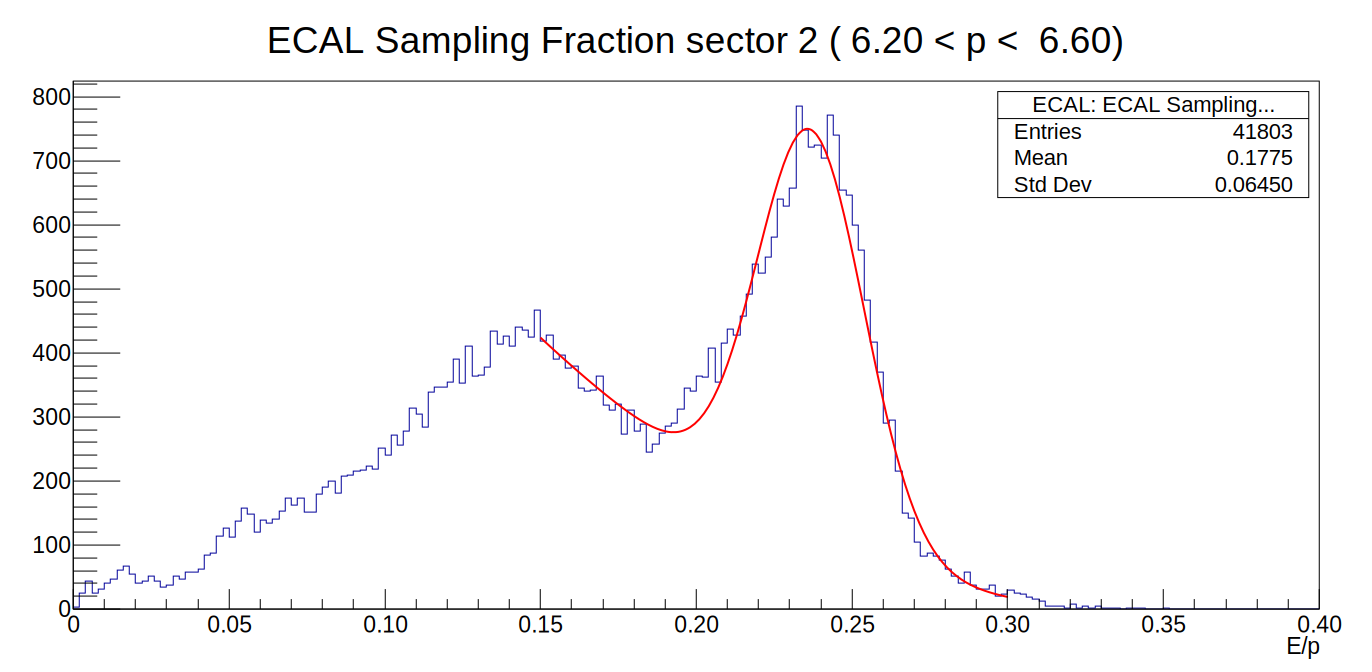
\includegraphics[width=\textwidth]{31sf_1d_plot2.pdf}}
                }
            \end{figure}
        \end{center}
    \end{column}

    \end{columns}

    \vspace{-9pt}

    \scriptsize{\textit{
        \ef{$E_{dep}/p$} distribution for two $0.4$ GeV \ef{$p$} bins for $e^-$ in the CLAS12 Electronic Calorimeter.
        The fit only covers from $0.15$ to $0.30$ based on what we expect for $e^-$ from theory.
    }}
\end{frame}

